The numbers below coorrespond to each company's planet.

\begin{center}
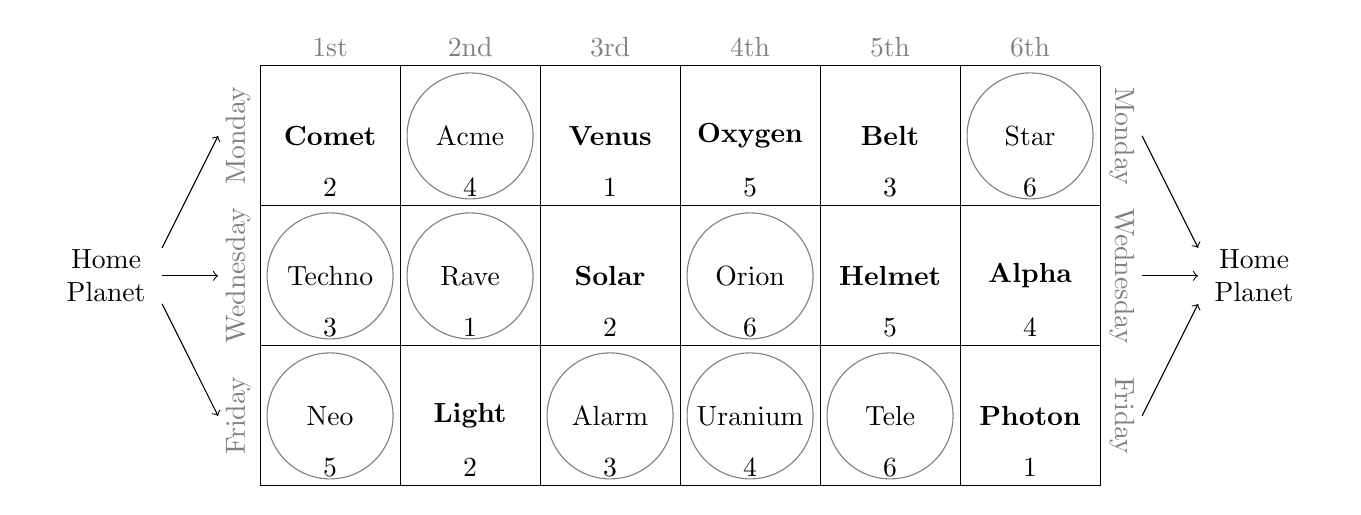
\begin{tikzpicture}[x=0.7in,y=0.7in]
\fill[white] (-4,0) rectangle (4,3);
\draw[step=1,thin] (-3,0) grid (3,3);

\node[text width=5em,align=center] at (-4.1,1.5) {Home\\Planet};
\node[text width=5em,align=center] at (4.1,1.5) {Home\\Planet};
\draw[->] (-3.7,1.7) -- (-3.3,2.5);
\draw[->] (-3.7,1.5) -- (-3.3,1.5);
\draw[->] (-3.7,1.3) -- (-3.3,0.5);
\draw[<-] (3.7,1.7) -- (3.3,2.5);
\draw[<-] (3.7,1.5) -- (3.3,1.5);
\draw[<-] (3.7,1.3) -- (3.3,0.5);

\node[color=gray,anchor=east] at (-3,2.5) {\rotatebox{90}{Monday}};
\node[color=gray,anchor=east] at (-3,1.5) {\rotatebox{90}{Wednesday}};
\node[color=gray,anchor=east] at (-3,0.5) {\rotatebox{90}{Friday}};
\node[color=gray,anchor=west] at (3,2.5) {\rotatebox{270}{Monday}};
\node[color=gray,anchor=west] at (3,1.5) {\rotatebox{270}{Wednesday}};
\node[color=gray,anchor=west] at (3,0.5) {\rotatebox{270}{Friday}};

\node[color=gray,anchor=south] at (-2.5,3) {1st};
\node[color=gray,anchor=south] at (-1.5,3) {2nd};
\node[color=gray,anchor=south] at (-0.5,3) {3rd};
\node[color=gray,anchor=south] at (0.5,3) {4th};
\node[color=gray,anchor=south] at (1.5,3) {5th};
\node[color=gray,anchor=south] at (2.5,3) {6th};

\draw[color=gray] (-1.5,2.5) circle (0.45);
\draw[color=gray] (2.5,2.5) circle (0.45);
\draw[color=gray] (-2.5,1.5) circle (0.45);
\draw[color=gray] (-1.5,1.5) circle (0.45);
\draw[color=gray] (0.5,1.5) circle (0.45);
\draw[color=gray] (-2.5,0.5) circle (0.45);
\draw[color=gray] (-0.5,0.5) circle (0.45);
\draw[color=gray] (0.5,0.5) circle (0.45);
\draw[color=gray] (1.5,0.5) circle (0.45);

\node at (-2.5,2.5) {\textbf{Comet}};
\node at (-0.5,2.5) {\textbf{Venus}};
\node at (0.5,2.5) {\textbf{Oxygen}};
\node at (1.5,2.5) {\textbf{Belt}};

\node at (-0.5,1.5) {\textbf{Solar}};
\node at (1.5,1.5) {\textbf{Helmet}};
\node at (2.5,1.5) {\textbf{Alpha}};

\node at (-1.5,0.5) {\textbf{Light}};
\node at (2.5,0.5) {\textbf{Photon}};

%SOLUTION
\node at (-1.5,2.5) {Acme};
\node at (2.5,2.5) {Star};
\node at (-2.5,1.5) {Techno};
\node at (-1.5,1.5) {Rave};
\node at (0.5,1.5) {Orion};
\node at (-2.5,0.5) {Neo};
\node at (-0.5,0.5) {Alarm};
\node at (0.5,0.5) {Uranium};
\node at (1.5,0.5) {Tele};
\node[above] at (-2.5,2) {2};
\node[above] at (-1.5,2) {4};
\node[above] at (-0.5,2) {1};
\node[above] at (0.5,2)  {5};
\node[above] at (1.5,2)  {3};
\node[above] at (2.5,2)  {6};
\node[above] at (-2.5,1) {3};
\node[above] at (-1.5,1) {1};
\node[above] at (-0.5,1) {2};
\node[above] at (0.5,1)  {6};
\node[above] at (1.5,1)  {5};
\node[above] at (2.5,1)  {4};
\node[above] at (-2.5,0) {5};
\node[above] at (-1.5,0) {2};
\node[above] at (-0.5,0) {3};
\node[above] at (0.5,0)  {4};
\node[above] at (1.5,0)  {6};
\node[above] at (2.5,0)  {1};
\end{tikzpicture}
\end{center}

Using the first letters of the filled-in company names, the solution
\texttt{ASTRONAUT} is revealed.
